
\section{ Наблюдения одиночных черных дыр и черных дыр в двойных системах звездных масс.}

Дать однозначное определение черной дыры не просто. Для астрономии \textbf{Черная дыра} - это компактный массивный объект, обладающий некими внешними свойствами: нет проявления признаков наличия поверхности, недоступные для наблюдения недра. Именно по такому определению и пытаются искать эти объекты, однако доказать, что это именно черная дыра - сложная задача.

С точки зрения астрономии черные дыры существуют, они являются самым простым, самым консервативным объяснением для объекта, который не проявляет признаков наличия поверхности.

\subsection{Одиночная черная дыра}

При попытке посмотреть на черную дыру мы сталкиваемся с очевидной проблемой: мы не видим её саму. Нам необходимо исследовать то, на что она влияет своей гравитацией. Есть два основных способа:

\begin{enumerate}
	\item Изучение аккреции
	\item Микролинзирование
\end{enumerate}

Вокруг черной дыры есть вещество, оно неизбежно притягивается к ней, однако чтобы оно могло начать выделять энергию оно должно быть из газа(а не из пыли), и не всегда темп аккреции(кол-во вещества, падающего на черную дыру) велик для достаточного энерговыделения, чтобы мы смогли задетектировать это.

Микролинзирование - наблюдение увеличения блеска видимых источников \textbf{за} черной дырой. При этом, если принять, что все объекты движутся с ~одной скоростью или скорости лежат в каких-то адекватных пределах, то длительность этого эффекта тем больше, чем больше масса нашей линзы(если в случае экзопланет эффект длился ~сутки, то тут можно наблюдать эффект ~год и более). Получая отсюда оценку массы, мы можем посмотреть в точку и узнать: "А видим ли мы что-то в этом месте?". Если масса порядка звездной, но ничего нет, это в первую очередь черная дыра.

\subsection{Черная дыра в двойной системе}

Когда вместе с черной дырой вращается детектируемый объект(или еще одна черная дыра), задача существенно упрощается, потому что появляются различные явления, если у космического объекта есть компаньон-черная дыра.

В двойной системе можно использовать \href{https://en.wikipedia.org/wiki/Binary_mass_function}{функцию масс}, чтобы оценить массу невидимой компоненты по наблюдаемым величинам: периоду движения и максимальной лучевой скорости видимой компоненты(hence, метод похож на детектирование экзопланеты, но скорость видимой компоненты здесь больше).

Когда система компактная, то видимый источник(звезда) может заполнить полость Роша и вещество начнет аккрецировать на черную дыру, начиная излучать в рентгене. Первым хорошим кандидатом была система в созвездии Лебедь, название Лебедь X-1(Cyg X-1 на рисунке \ref{fig:13_compact})

\begin{figure}[H]
	\centering
	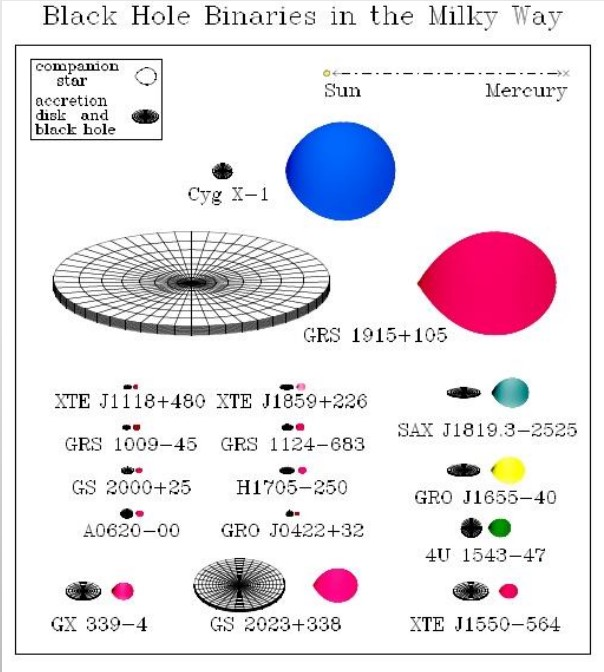
\includegraphics[width=0.7\linewidth]{13_compact}
	\caption{Примеры и масштабы рентгеновских источников}
	\label{fig:13_compact}
\end{figure}

Как мы можем утверждать, что внутри аккреционного диска расположена именно черная дыра?

\begin{enumerate}
	\item В отличии от нейтронных звезд, у которой есть поверхность и магнитное поле, а также она вращается, мы бы наблюдали "пульсации" излучения, связанные с этим вращением нашего диполя-нейтронной звезды. Однако пульсации могут не быть и у нейтронных звезд со слабым магнитным полем(про это задача в дз5, задача 1).
	\item Особенности излучения ЧД. Например, в отличии от нейтронной звезды, у которой вещество на радиусе остановки образует некий пограничный слой, растекаясь по поверхности и это можно детектировать в спектре мощности, у черной дыры внутренняя граница аккреционного диска определяется самой внутренней устойчивой круговой орбитой и нет схожих проявлений в спектре.
	\item Оценкой массы можно исключить из рассмотрения нейтронные звезды, потому что их масса не может превышать ~3 масс Солнца.
\end{enumerate}

Некоторые из таких двойных систем являются \textbf{Рентгеновскими новыми}, в которых аккреция является нестационарной, и выброс энергии идет вспышками. Они дают оценку получше, потому что есть две фазы: когда видно в основном яркий аккреционный диск(вспышка), и когда видно тусклый красный карлик(спокойное состояние; из рисунка \ref{fig:13_compact}, именно КК обычно входят в состав такой системы), поэтому оценка на массу получается лучше.

Однако и нейтронные звезды могут быть такими транзиентными(непостоянными) источниками, но отличить их можно по минимальной светимости в этой спокойной фазе. В этой фазе всё равно есть небольшое перетекание массы с КК, но из-за отсутствие поверхности у черной дыры она не эффективно перерабатывает это небольшое кол-во материала в энергию, в отличии от нейтронной звезды, которая своей магнитосферой размазывает вещество по поверхности и тем самым не может светить тусклее черной дыры.

К тому же, у систем с нейтронной звездой имеется явление 'Рентгеновского барстера' - если кратко, это накапливание вещества у поверхности звезды, после которого идет вспышка(из-за термоядерной реакции на поверхности) в рентгеновском диапазоне. У некоторых систем такое не наблюдается, и простое объяснение - там нет поверхности, где бы накапливалось вещество, то есть мы имеем дело с черной дырой.

\begin{figure}[H]
	\centering
	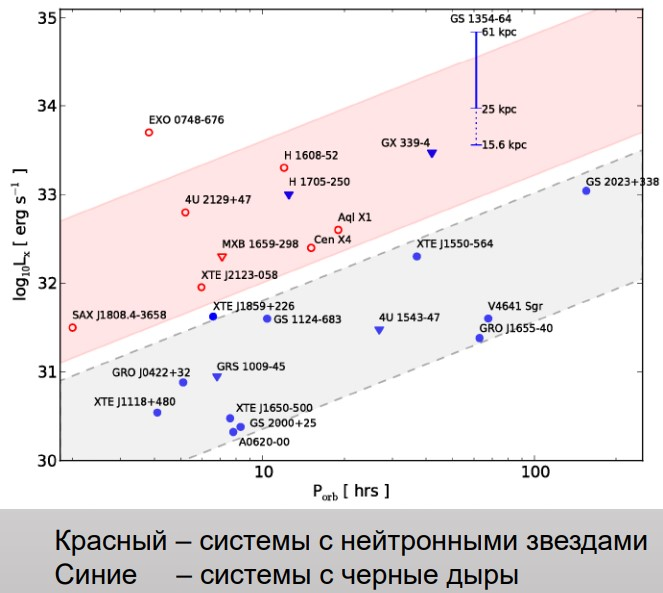
\includegraphics[width=0.7\linewidth]{13_xray_new}
	\caption{Светимость систем с НЗ и ЧД}
	\label{fig:13_xray_new}
\end{figure}

\subsection{Двойная система из черных дыр}

Интересным случаем является двойная система двух черных дыр, а именно явление \textbf{слияния черных дыр}, детектировать которое мы можем по гравитационным волнам, характерная длина волн которых порядка этой системы дыр, то есть величины порядка 100 км и более).
